\documentclass[a4paper,11pt,twoside,openright]{book} % Type du document

% compile using : pdflatex, bibtex, pdflatex, pdflatex

% +---------------------------------------------------------------+
% | Language
% +---------------------------------------------------------------+
\usepackage[T1]{fontenc}
\usepackage[utf8]{inputenc}
\usepackage[english]{babel}

\newif\ifisconfidential    \isconfidentialfalse
% \newif\ifisconfidential	\isconfidentialtrue

\newif\ifisdraft\isdrafttrue
% \newif\ifisdraft\isdraftfalse

\usepackage{hyperref}
\hypersetup{
    colorlinks=true,
    linkcolor=black,
    filecolor=black,
    urlcolor=blue,
    pdftitle={report},
    pdfpagemode=FullScreen,
}

% +---------------------------------------------------------------+
% | Parameters
% +---------------------------------------------------------------+

\newcommand{\docLogo}{template/logo_unibern.png}
% \newcommand{\docLogo}{template/logo_unifr.png}

\newcommand{\docTitle}{TODO TITLE}
\newcommand{\docSubtitle}{TODO SUBITLTE}%laisser vide si pas de sous-titre
\newcommand{\docAuthor}{Mario Amos}

\newcommand{\docAcademicYears}{2025-2026}

\newcommand{\docDpt}{University of Bern}
\newcommand{\docFiliere}{Faculty of Science}
\newcommand{\docOrient}{Bioinformatics and Computational Biology}

\newcommand{\docDate}{Bern, \today}

% uncomment if confidential / comment if not confiential
% \isconfidentialtrue

% +-[set path]-------------------------------------+
\usepackage{template/template}
\usepackage{template/style}
\usepackage{template/macros}

%\graphicspath{images/}
\usepackage{hyperref}%Doit etre le dernier package

\begin{document}

    \frontmatter
    \pagestyle{empty}

    % TITLE
% +---------------------------------------------------------------+

\thispagestyle{empty}

\begin{minipage}[t]{6cm}
    \vspace{0pt}%usefull to align top
    \includegraphics[width=3cm]{\docLogo}
\end{minipage}\hfill\begin{minipage}[t]{10cm}%
    \vspace{0pt}%usefull to align top
    \small%
    \begin{flushright}%
        \docDpt\\
        \docFiliere\\
        \docOrient
    \end{flushright}
\end{minipage}

\vspace{7cm}

\begin{center}

{\Huge \bfseries \docTitle}

  \ifthenelse{\isempty{\docSubtitle}}%
        {empty}%empty
    {\Large \docSubtitle}%not empty
\end{center}
    
\vspace{5cm}

\normalsize
\begin{center}
    \begin{tabular}{r@{\hskip 13mm}l}
        \textbf{Student} & \docAuthor \\[0.1cm]
        \textbf{Study programm} & \docOrient \\[0.1cm]
        \textbf{Academic year} & \docAcademicYears \\[0.1cm]
    \end{tabular}
\end{center}


\vspace{1cm}

\begin{flushright}
    \docDate
\end{flushright}

\vspace{0cm}

\cleardoublepage   

\cleardoublepage

% Abstract
% +---------------------------------------------------------------+
\thispagestyle{plain}
\chapter{Abstract}
\label{ch:abstract}


% Authentification
% +---------------------------------------------------------------+

% \chapter{Authentification}
% \thispagestyle{plain}

% The undersigned, \docAuthor, hereby attests to having carried out this work and to having used
% no other source than those expressly mentioned.

% \vspace{2cm}

% \noindent \docDate

% \vspace{3cm}

% \begin{flushright}
%     \begin{minipage}{7cm}
%         {\docAuthor}
%     \end{minipage}\hfill
% \end{flushright}

\cleardoublepage

% TOC
% +---------------------------------------------------------------+
    \pagestyle{plain}
    \hypersetup{
        citecolor=blue,
        linkcolor=black
    }
    \markboth{Table of contents}{}
    \tableofcontents
    \label{endoftoc}
    \clearpage
    \hypersetup{
        citecolor=blue,
        linkcolor=blue
    }


% Content
% +---------------------------------------------------------------+

    \mainmatter
    \global\Introfalse
    \pagestyle{plain}

    \chapter{Introduction}
\label{ch:intro}


\section{Demo}

\subsection{2 column}

\begin{multicols}{2}
[
    All human things are subject to decay. And when fate summons, Monarchs must obey.
]

    \blindtext

    \blindtext
\end{multicols}

\subsection{Code listing}

\begin{lstlisting}[language=bash]
[mamos@binfservas31 mamos]$ apptainer exec /containers/apptainer/subread_2.0.6.sif featureCounts -v
\end{lstlisting}

\begin{lstlisting}
    featureCounts v2.0.6
\end{lstlisting}

\subsection{Table and footnote}

\begin{longtable}[c]{|l|l|l|l|}
    \hline
    Software & Version & Module or container & Container path\footnotemark{} \\
    \hline
    \endfirsthead

    \hline
    Software & Version & Module or container & Container path\footnotemark[\value{footnote}]{} \\
    \hline
    \endhead

    \multicolumn{4}{r}{\small \it The table continues on the next page} \\
    \normalsize
    \endfoot
    \hline
    \caption{Table of used software and versions}
    \endlastfoot

    FastQC & 0.11.9-Java-11 & Module &  -\\
    FastQC & 0.11.9-Java-11 & Module &  -\\
    fastp & 0.23.4-GCC-10.3.0 & Module &  -\\
    featureCounts & 2.0.6 & Container &  \lstinline!subread_2.0.6.sif! \\
    samtools & 1.20 & Container &  \lstinline!hisat2_samtools_408dfd02f175cd88.sif!\\
    hisat2 & 2.2.1 & Container &  \lstinline!hisat2_samtools_408dfd02f175cd88.sif!

    \footnotetext{On the cluster, all the path mentioned are located in /containers/apptainer/}
    \label{table:softwaresVersions}
\end{longtable}

\subsection{Figure}

\begin{figure}[h]
    \centering
    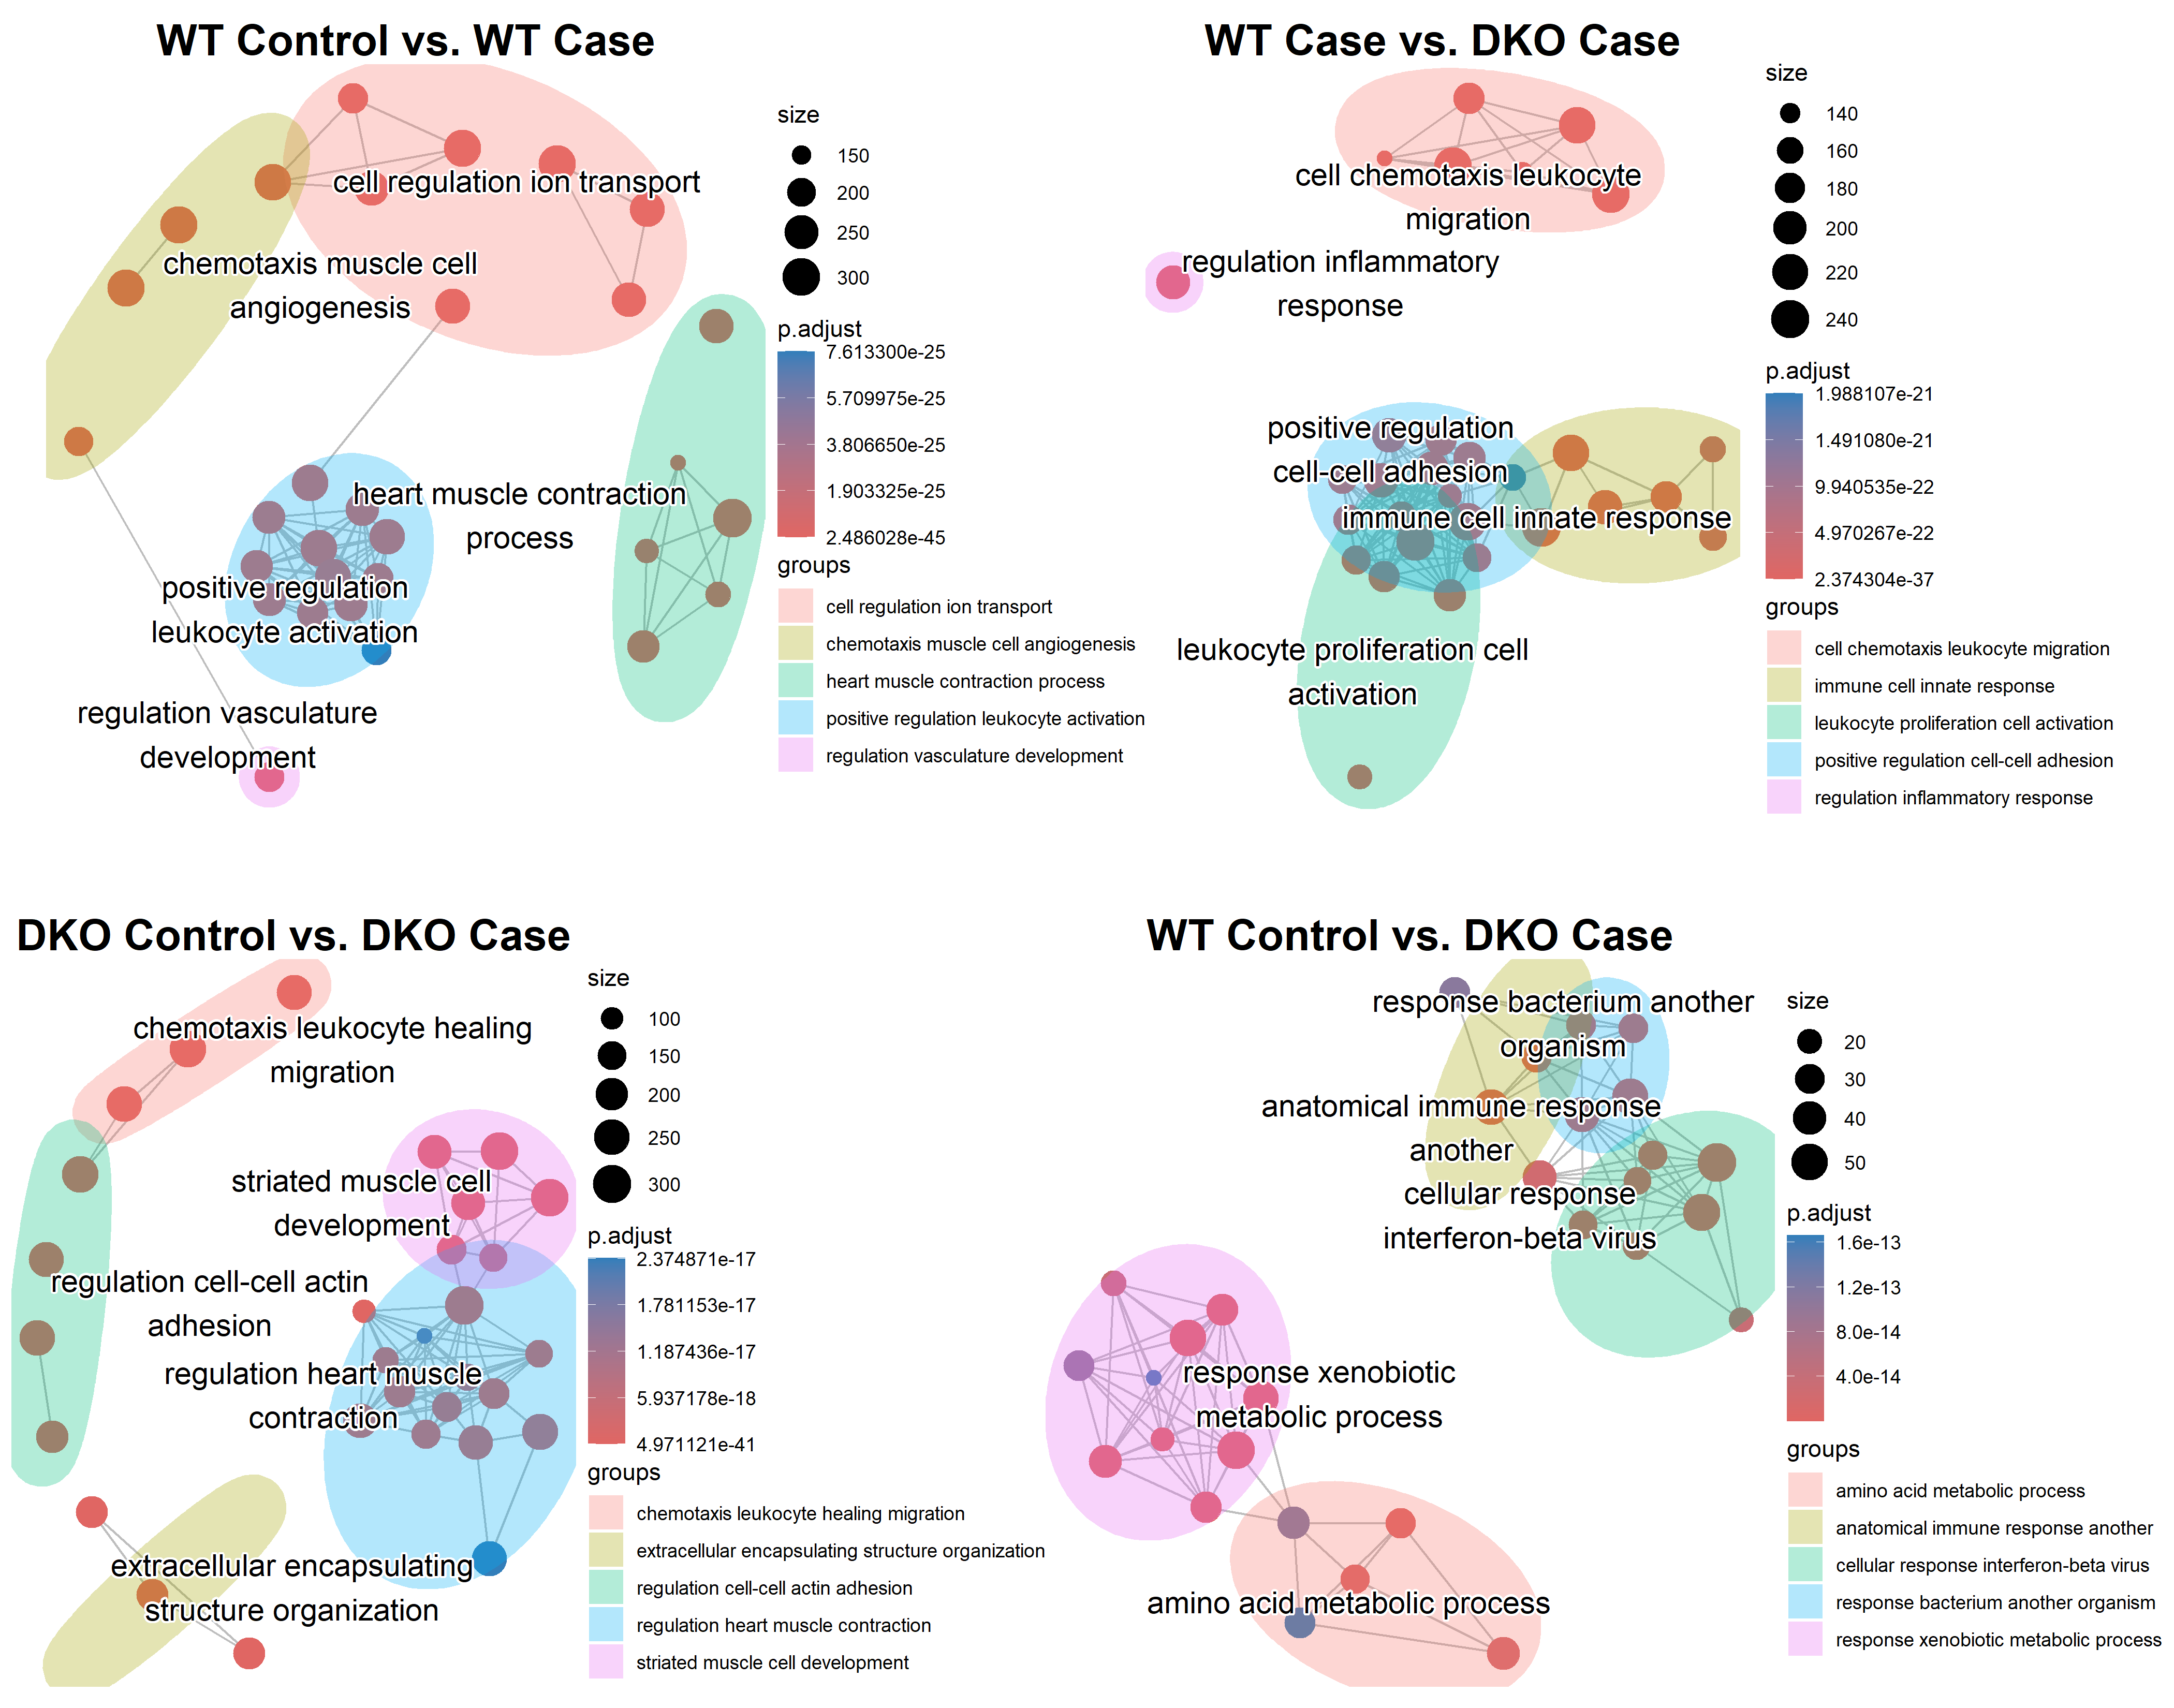
\includegraphics[width=1\linewidth]{figures/go_summary.png}
    \caption{Enrichement map from overrepresentation analysis}
    \label{fig:goSummary}
\end{figure}

    \chapter{Material and methods}
\label{ch:materialAndMethods}

    \chapter{Results}
\label{ch:results}


    \chapter{Conclusion}
\label{ch:conclusion}

\section{Discussion}

\section{Future Work}


% Supplentary materials

% +---------------------------------------------------------------+
    \cleardoublepage
    \phantomsection
    \addcontentsline{toc}{chapter}{Bibliography}
    \markboth{Bibliography}{Bibliography}
    \bibliographystyle{IEEEtran}
    \bibliography{biblio}
    \nocite{*} %ajoute tout ce qu'il y a dans le bibtex

    \hypersetup{
        citecolor=blue,
        linkcolor=black
    }
    \phantomsection
    \listoffigures
    \addcontentsline{toc}{chapter}{Table of figures}
    \markboth{Table of figures}{Table of figures}

    \phantomsection
    \listoftables
    \addcontentsline{toc}{chapter}{List of tables}
    \markboth{List of tables}{List of tables}
    \hypersetup{
        citecolor=blue,
        linkcolor=blue
    }

    \phantomsection
    \cleardoublepage
    \appendix
    \chapter{Source code}

All scripts used for data processing and analysis were version-controlled and hosted on a public GitHub repository \cite{GitHub}. This ensures the workflow is documented, transparent, and accessible for future replication.

Repository link : \href{https://github.com/aoiram/TODO}{https://github.com/aoiram/TODO}


% Annexes
% +---------------------------------------------------------------+
    \appendix

    % \includepdf[pages=-, scale=1, angle=90,  offset=0 0]{HEIG-TB-CARAMLLM/doc_latex/tb-planification.pdf}

\end{document}